%%%%%%%%%%%%%%%%%%%%
\section{Discussion}
\label{sec:cryptobinary-discussion}

We now provide a discussion backed by our evaluation results and examination of existing work and implemented tools, delving into broader issues that we discovered.  This includes discussing additional overarching future research directions and key areas where improvements can be made moving forward.

%Within this particular section, we aim to delve deeper into the issues and potential avenues for further research that we have identified based on our comprehensive evaluation results. With consideration of the evaluation results, we found our some issues to detect cryptographic function in binary. Meanwhile, we have discovered several key areas where improvements could be made.


\subsection{Approaches to Algorithm Detection in Tools}

%\emph{R4: Can the same tool perform similarly well across different algorithms?}
% \begin{figure}[h]
%   \includegraphics[width=0.5\linewidth,keepaspectratio]{./images/evaluate_tool.jpg}
%   \caption{Untitled}
%   \label{fig:evaluate_tool}
  
% \end{figure}

We start by discussing the detection results of a single tool for different algorithms. We opted to evaluate 12 distinct algorithms (AES, DES, ECC, MD5, RC4, RC5, RSA, SHA-1, SHA-256, TEA, XTEA, and XXTEA) along with our microbenchmarks, various libraries, and a large-scale project.

Based on our evaluation (see \autoref{tab:cryptobinary-benchmarks}), we found that PEiD KANAL, SignSrch, and Where's Crypto can detect most algorithms we selected. This was somewhat expected as Where's Crypto is a more modern detection tool. HCD demonstrated average performance in our evaluation results.
%but it is the only tool that can detect ECC. 
Nonetheless, we came across cases where tools did not detect cryptographic functions they were expected to identify, indicating potential need to enhance detection accuracy.

\begin{takeaway}
\textbf{Future Research:} Current tools seemingly employ various (often distinct) approaches compared to one another. Many of these tools also provide developers with the opportunity to expand and enhance their detection capabilities. Therefore, future research could focus on improving existing technologies within individual tools and existing approaches to achieve broader applicability with higher detection rates, and to make it so that users do not need to use different tools to best identify different algorithms.
\end{takeaway}

\subsection{AI/ML Approach}
Artificial intelligence and machine learning (AI/ML) have been extensively applied across various domains to address complex problems. Previous works, like CryptoKnight, have utilized machine learning techniques for cryptographic function detection. However, in our evaluation, we found that these tools did not exhibit satisfactory performance. We attribute this issue not to the approach itself, but rather to the fact that these tools typically only offer a demonstration to showcase the potential application of AI/ML in this field. The main problem lies in the lack of sufficient signatures or analysis provided by these tools, which is likely the primary reason for their low performance.
\begin{takeaway}
\textbf{Future Research:} 
While current AI/ML based tools demonstrate the feasibility of utilizing AI/ML in cryptographic function detection, they fall short in providing the robust and comprehensive signature or analysis capabilities necessary for accurate detection.  These seem like promising future research directions.
\end{takeaway}

\subsection{Lack of Support for Modern Cryptographic Algorithms}

Many modern cryptographic algorithms, such as general Elliptic-Curve Cryptography (ECC) and more specifically ECDSA and ECDHE, have found widespread use in diverse applications~\cite{harkanson2017applications} due to their advantages in terms of smaller private key size and improved efficiency at equivalent or higher security levels. ECDSA is utilized in a number of areas, including electronic healthcare, banking, commerce, and vehicles \cite{al2019efficient}, and is currently supported by most major libraries, including cryptlib, Crypto++, libgcrypt, LibreSSL, and OpenSSL.
However, our evaluation reveals that existing work lacks the ability to find such modern algorithms. As such, this could be a rich area for future development and improvement. 
\begin{takeaway}
\textbf{Future Research:} 
As the prevalence of applications adopting ECC continues to rise, the ongoing development of cryptographic function detection has led to a disconnect between the outcomes of these efforts and the real-world applications that people are eager to test, leading to an important direction for future research.
\end{takeaway}

% Besides the evaluation metrics we evaluated in Section \ref{subsec:metrics} The false positive may affected by the 
% This underscores the importance of recognizing that the implementation of cryptographic functions can significantly impact detection ability. The presence of optimizations or deviations from the standard algorithm can also lead to false negatives in the detection process.
\subsection{Comparative Detection of Similar Algorithms Across Various Tools}
% \begin{figure}[h!]
%   \includegraphics[width=0.5\linewidth,keepaspectratio]{./images/evaluate_algo.jpg}
%   \caption{Untitled}
%   \label{fig:evaluate_algo}
%\emph{R3: Are some algorithms easier to detect compared to others?}

% \end{figure}
Our evaluation helps provides insights from an algorithmic perspective on how well different tools can detect the same cryptographic algorithm. In our evaluation, we test the tools' abilities to find cryptographic functions in different settings (optimization flags, compilers, etc.). \autoref{fig:cryptobinary-algo_easy} shows the percentage of algorithms that can be successfully detected by a tool across all evaluation experiments that we ran.
We can see that TEA, RC5, and SHA can be successfully detected in most experiments. However, AES, and MD5 can only be found in a few experiments, with algorithms like RC4 and ECC not even being detected at all.

\begin{figure}[t]
    \centering
  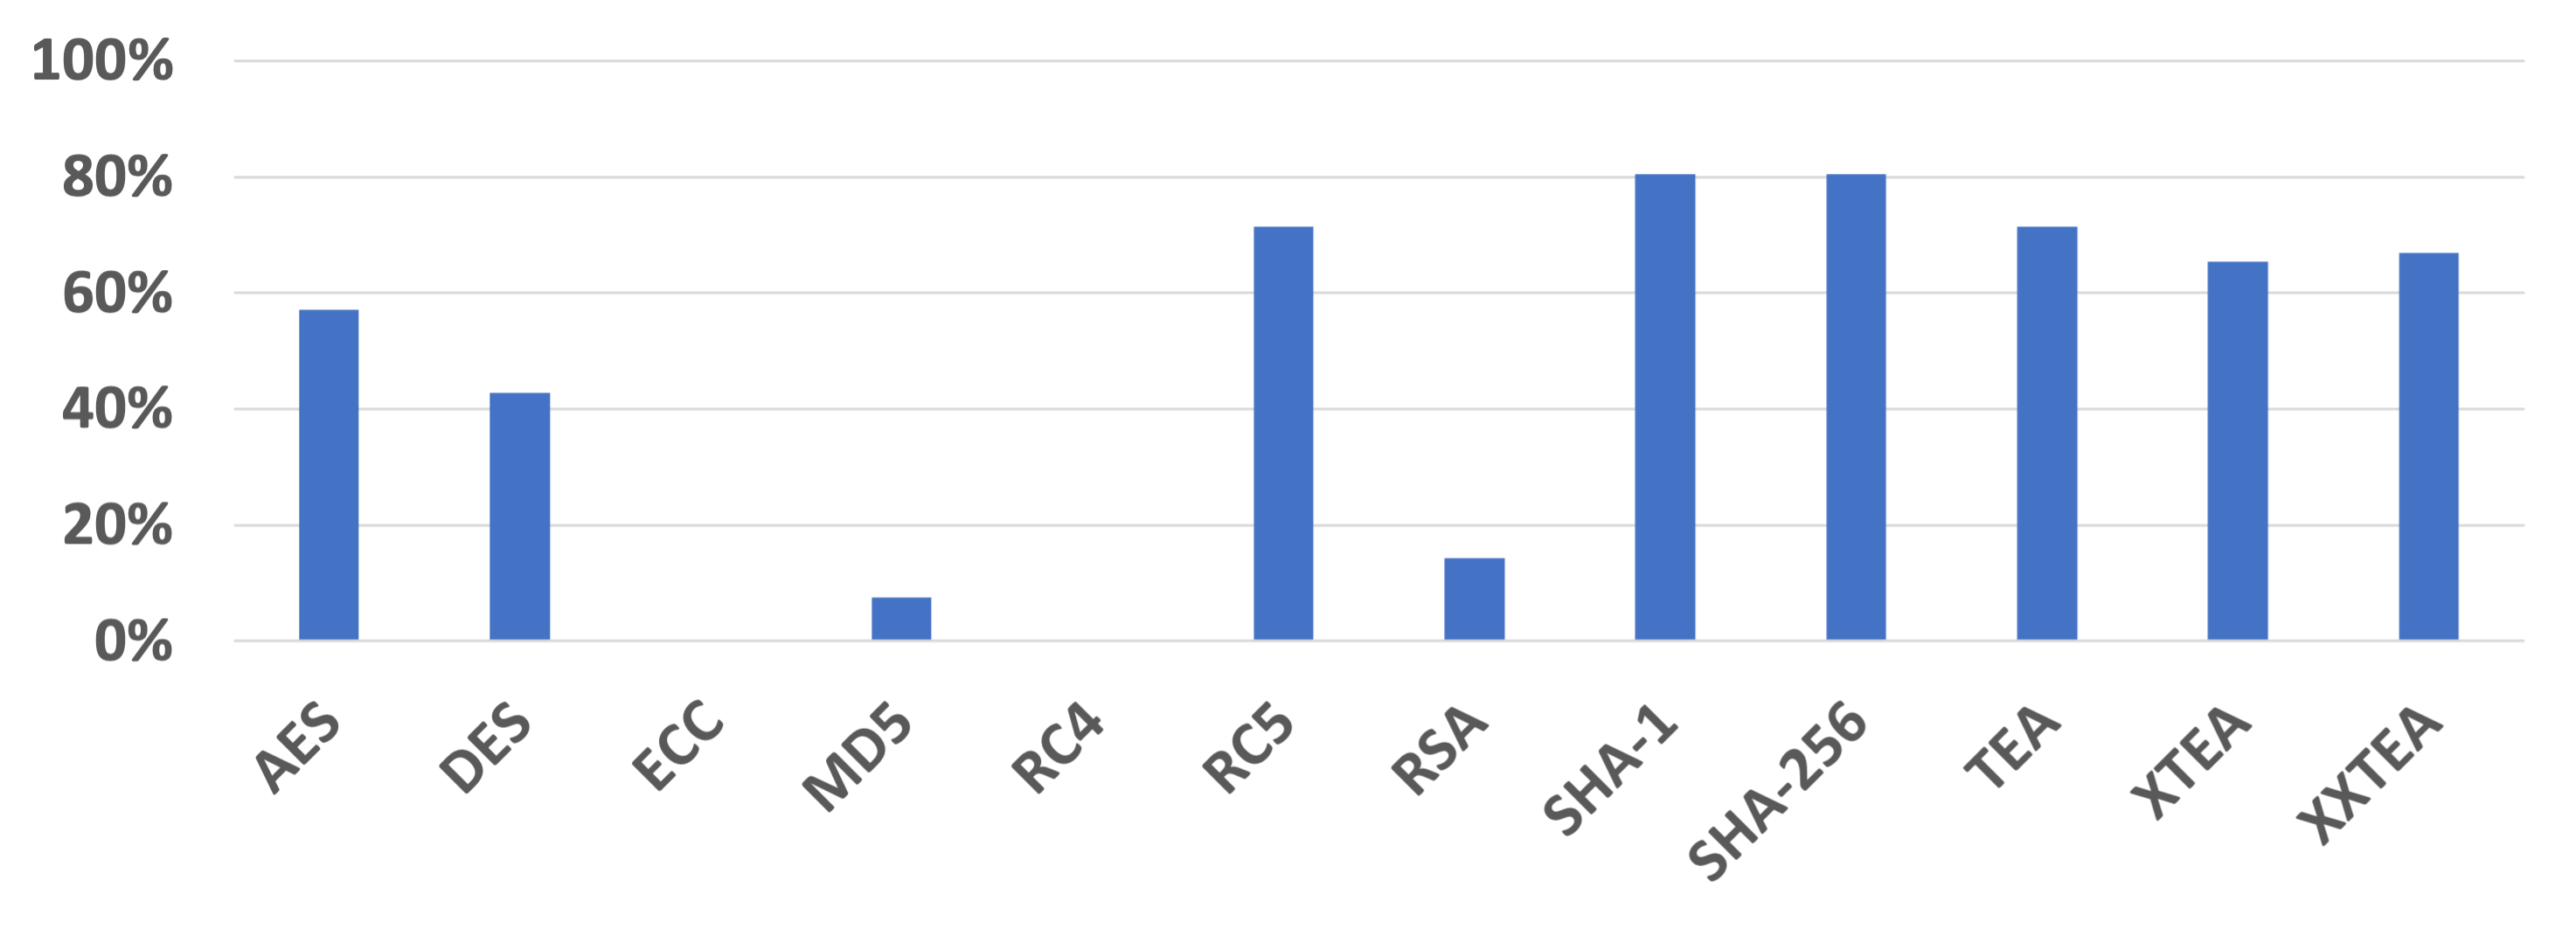
\includegraphics[width=0.95\linewidth,keepaspectratio]{ch-cryptobinary/figure/algoeasy.png}
  \caption{Detection percentage by algorithm across all tools}
  \label{fig:cryptobinary-algo_easy}
\end{figure}

From our observations, it is not evident that there exists a consistent rule governing the ease of detecting specific categories of cryptographic functions. For instance, when considering two hash functions, MD5 and SHA, we note markedly different results. Even within the same family we find variations; TEA and RC5, both belonging to the block cipher family, exhibit detectability, while DES, another block cipher, proves more challenging to detect.

%\noindent\fbox{%
    %\parbox{\textwidth}{%
        %Future Research Question: Some cryptographic algorithms are more challenging to detect than others, as indicated by our evaluation results. Notably, we have not observed a distinct pattern suggesting that algorithms within a specific category consistently present greater difficulty in detection. Therefore, the future research could focus on how to detect cryptographic algorithms that appear to be harder to identify or investigate the underlying factors that contribute to variations in the detectability of algorithms within the same category.
    %}%
%}

\begin{takeaway}
\textbf{Future Research:} Some cryptographic algorithms appear to be more challenging to detect than others. However, we have not observed a distinct pattern suggesting that algorithms within a specific category consistently present greater difficulty in detection. Therefore, future research could focus on how to detect cryptographic algorithms that appear to be harder to identify or investigate the underlying factors that contribute to variations in the detectability of algorithms within the same class.
\end{takeaway}



%\subsection{Leveraging General Binary Analysis Techniques}
%\label{leverage-binary}
%%\noindent\fbox{%
    %%\parbox{\textwidth}{%
        %%Future Research Question: 
    %%}%
%%}
%Binary code similarity analysis is an active area of research in the software community. There has been a plethora of research~\cite{david2017similarity, saebjornsen2014detecting, liu2018eclone, chandramohan2016bingo, mckee2019software, ding2019asm2vec, ming2017binsim, xu2017neural} to compare two or more binaries to identify their similarities or variances.  
%
%BLEX~\cite{egele2014blanket} proposed a dynamic similarity testing system based on the novel technique of blanket execution 
%consisting of seven binary code semantics extractor. Tinbergen~\cite{mckee2019software} presented a framework which infers function semantics through program state change. DyCLINK~\cite{su2016code} used dynamic dependency graph to capture code behavior at the instruction level and then
%performed similarity analysis via computing an isomorphism between sub graphs.
%There are also some notable NLP based binary similarity analysis techniques~\cite{ding2019asm2vec, xu2017neural}.
%Asm2Vec~\cite{ding2019asm2vec} is a representation learning model that learns latent lexical semantics between
%tokens and represents an assembly function as an internally weighted mixture of collective semantics.
%Gemini~\cite{xu2017neural} proposes a neural network-based approach to compute the embedding, i.e., a numeric vector, based on the control
%flow graph of each binary function and then performs the similarity detection via measuring the distance between the embeddings for two functions.

%\begin{takeaway}
%\textbf{Future Research:}
%Although binary similarity research is very similar to some cryptographic function identification approaches and shares a similar set of challenges, cryptographic detection research has a much more limited scope of work and techniques thus far.
%Hence, an avenue for future research is investigating the use of binary similarity techniques in this more targeted space.  
%\end{takeaway}


% \subsection{Discussion of Evaluation Results}
% Based on our evaluation, we found that most of the cryptographic detection tools have similar performance such as

% \begin{itemize}[leftmargin=*]
%     \setlength{\itemsep}{0pt}
%     \setlength{\parskip}{0pt}
%         \item Cannot detect RSA and modern cryptohtrapicy algorithm ECC in binary
%         \item Optimization flag and compiler do not affect the detetcion results in SHA (except for Signsrch) and TEA
%         \item Can only detect MD5 compiled with no flag or $\O0$ in GCC
% \end{itemize}

% In the course of our evaluation, we have encountered instances of false negatives in certain cryptographic detection tools. For instance, both DRACA and FindCrypt2 assert their ability to detect DES functions within binaries. However, we were unable to replicate this result even when using a standard DES implementation without any obfuscation during compilation.

\subsection{User Experience}

Considering the experience and insights we have garnered from our evaluation process, we believe that discussing the developer experience is also an intriguing topic, in terms of how developers interact with these tools and their ease of use.

Older cryptographic detection tools, such as DRACA, PEiD KANAL, and SignSrch, do not require developers to compile and build the tools from source code. Developers can readily utilize these tools with supported operating systems. However, when compared to some better performing tools, these user-friendly alternatives exhibit lower performance and utility. For example, obfuscation can disturb the binary analysis process of Signsrch, leading to false negatives in the detection of certain cryptographic algorithms. Furthermore, DRACA struggles to accurately analyze packed executable programs, and consequently, it can only provide a rudimentary analysis outcome, despite its ease of use.

In addition to the aforementioned challenges, some tools pose difficulties for users due to technological complexity or data-related issues. Take, for instance, IDA Scope, Findcrypt2, and Where's Crypto, which all rely on IDA Pro. IDA Pro is not a free, open-source software, and these tools cannot be utilized by developers without it. Conversely, tools such as CryptoKnight and other machine learning-based techniques require users to provide substantial amounts of data, which further compounds the difficulty of using these tools. 

However, these tools generally exhibit superior performance when compared to user-friendly alternatives. For instance, CryptoHunt consistently yields accurate analysis results for identification within obfuscated programs. Where's Crypto, one of the most recent cryptographic detection tools, broadens the scope of analysis to encompass unfamiliar and proprietary cryptographic primitives, without relying on heuristics to select code fragments.

\subsection{Challenges for Future Research}
\label{subsec:cryptobinary-challenges}

%Identifying cryptographic functions has its own sets of challenges. 
Based on our evaluation, we have identified several challenges that make cryptographic function identification difficult.
In this subsection, we discuss some of these challenges, as we believe they may help inform future tool development and areas of research.

%%%%%%%%%%%%%%%%%%%%%%%%
\parhead{Obfuscation.} One of the major challenges in cryptographic function identification is obfuscation.
The initial purpose of obfuscation was to protect software intellectual
property~\cite{collberg1997taxonomy} from malicious reverse engineering
attempts. However, malware authors adopted obfuscation techniques as a way to
avoid detection. Various types of obfuscation techniques have been implemented
to thwart any form of detection. These obfuscation techniques can be primarily
categorized as: control-flow obfuscation, data obfuscation, and layout obfuscation.
For a variety of reasons, one might still wish to identify cryptographic code
even in the face of such obfuscation techniques, particularly given its prevalence nowadays.
%Malware authors mostly adhere to control-flow and data obfuscations.

Control-flow obfuscation is the most common type of obfuscation. A control-flow graph (CFG) \cite{CFG} embodies the graphical
representation of the flow of a program. To hinder CFG-based detection, malware authors introduce techniques such as including bogus control-flow \cite{li2021code}, control-flow flattening \cite{cfg_f}, and opaque predicates \cite{xu2018opaque}. 
Similar to control flow obfuscation, data obfuscation techniques, like data aggregation and data
splitting, attempt to hinder approaches based on input/output relationships. For example, one might split a single variable into two to prevent detection.
%\autoref{lst:data_splitting} shows an example of data
%obfuscation, and how one variable used in \autoref{lst:normal_program}
%can be split into two variables to prevent detection.  
%
%\lstset{language=C,
        %label=lst:normal_program,
        %float=h,
        %caption={Normal program},
        %captionpos=b,
        %showlines=true,
        %breaklines=true,
        %breakatwhitespace=true,
        %tabsize=2,basicstyle=\footnotesize}
%\hspace*{-1.1cm}
%\begin{lstlisting}
%int var1 = func1();
%int var2 = func2();
%
%while(condition statement) {
	%int p1 = var1 * var2;
	%int p2 = var1 + var2;
%}
%\end{lstlisting}%
%%\hfill
%%\hspace*{0.1cm}
%\vspace{5pt}
%
%\lstset{language=C,
        %label=lst:data_splitting,
        %float=h,
        %caption={Data splitting},
        %captionpos=b,
        %breaklines=true,
        %breakatwhitespace=true,
        %tabsize=2,basicstyle=\footnotesize}
%\begin{lstlisting}
%int var1 = func1();
%int var2 = func2();
%
%short var11 = (short) (var1 >> 16);
%short var12 = (short) (var1 & 0xffff);
%
%while(condition statement) {
    %int new_var = (int) ((var11 << 16) | (var12 & 0xffff););
%
    %int p1 = new_var * var2;
    %int p2 = new_var + var2;
%}
%\end{lstlisting}
Layout obfuscation~\cite{xu2020layered} scrambles the layout of a program's instructions while keeping the original syntax intact. Layouts can be obfuscated by adding meaningless classifiers, stripping redundant symbols, separating related code, as well as adding junk code.

%%%%%%%%%%%%%%%%%%%%%%%%%%%%%%%%%%%%%

\parhead{Implementation Variation.} Despite having a well-defined specification, cryptographic algorithms can be implemented in a number of
ways while still achieving the same result.  In addition, cryptography is not always implemented correctly or exactly to spec.
For example, buggy implementations of the TEA algorithm
were found~\cite{calvet2012aligot} in malware such as Storm Worm and Silent Banker.
Hence, even if a detection approach can find an ideal implementation of an algorithm, there is no
guarantee it can also detect all the implementation variations
of the same algorithm. 
%We believe it is valuable (but challenging) to be able to identify both intended implementation variations, as well as as incorrect (but close) ones.
Our evaluations in this space are discussed in \autoref{subsec:cryptobinary-algo-version} and \autoref{subsec:cryptobinary-algo-version1}.

%%%%%%%%%%%%%%%%%%%%%%%%%%%%%%%%%%%%%%%%%%%%%%%%%%%

\parhead{Differences in Cryptographic Functions.} There are fundamental differences in different classes of cryptographic algorithms.
Cryptographic features (see \autoref{sec:cryptobinary-features}) present in one algorithm may not be present in others.
For instance, the data avalanche effect~\cite{li2012cipherxray} which says that an insignificant change in the input parameters can
make significant differences in the output, works well for identifying block ciphers. In the case of stream ciphers, there are
no such observations like data avalanching. Tools must be designed to account for these differences if they wish to identify broad classes of algorithms.

%%%%%%%%%%%%%%%%%%%%%%%%%%%%%%%%%%%%%%%%%%%%%%%%%%%

\parhead{Compilers.} The choice of compiler can significantly impact the binary structure of a program in various ways such as format, linking, inline functions, and compatibility with different architectures. The incorporation of anti-analysis techniques further adds to the complexity of cryptographic function detection. Consequently, working with different compilers can introduce numerous challenges. 
%Possessing knowledge about compiler behavior becomes essential for reverse engineers, security analysts, and detection tools to effectively identify cryptography within a binary program.
Our study (Section \ref{subsec:cryptobinary-effect-compiler}) demonstrates how a tool's detection capabilities can vary greatly depending on the compiler used.


%%%%%%%%%%%%%%%%%%%%%%%%%%%%%%%%%%%%%%%%%%%%%%%%%%%
\parhead{Comparison to General Binary Analysis.}
Binary code similarity analysis is an active area of research in the software community. There has been a plethora of research~\cite{david2017similarity, saebjornsen2014detecting, liu2018eclone, chandramohan2016bingo, mckee2019software, ding2019asm2vec, ming2017binsim, xu2017neural} to compare two or more binaries to identify their similarities or variances.  
While such generic binary analysis techniques can be leveraged in the detection of cryptographic functions, future researchers should bear in mind that detecting cryptographic functions in binary code remains a multifaceted challenge. Cryptographic algorithms exhibit significant variability in terms of complexity and implementation. They often involve intricate mathematical operations and employ various techniques such as bit manipulation, modular arithmetic, and logical operations. This complexity can pose difficulties in identifying cryptographic functions without specific knowledge of the algorithm being utilized.
%Furthermore, unlike some other types of functions or libraries that may have standardized signatures or calling conventions, cryptographic functions may lack easily recognizable patterns or signatures. They can be 
In addition, they can be implemented in diverse ways and may not adhere to consistent naming or calling conventions, rendering them more challenging to identify through static analysis alone.

%Additionally, detecting cryptographic functions in binary code constitutes a specialized domain within general binary analysis. Consequently, we anticipate a higher level of accuracy compared to detecting other types of functions in binary code.


%%Where's crypto, one of the latest cryptographic detection tool developed in 2021, provides an novel approach combines subgraph isomorphism with symbolic execution to find cryptographic algorithm in binary, but we did not discover a major performance improvement according to our evaluation results.

